\documentclass[0_main]{subfiles}

\begin{document}

\ifEn
    \section{Modified Secant Condition}
\else
    \section{修正セカント条件}
\fi
\label{sec:background_modified_secant}

\ifEn
    This section explains the modified secant condition, a modification of the standard secant condition used in quasi-Newton methods.
    The modified secant condition incorporates function value information in addition to gradient information, leading to more accurate Hessian approximations.
\else
    このセクションでは、準ニュートン法で使用される標準的なセカント条件の修正版である修正セカント条件について説明します。
    修正セカント条件は勾配情報に加えて関数値情報を取り込み、より正確なヘッセ行列の近似を実現します。
\fi

\ifEn
    \subsection{Standard Secant Condition}
\else
    \subsection{標準的なセカント条件}
\fi
\label{subsec:standard_secant}

\ifEn
    First, we review the standard secant condition used in quasi-Newton methods.
    Let $x_k$ and $x_{k+1}$ be two consecutive iterates generated by an optimization algorithm.
    To compute the next iterate, we need to update the approximate Hessian matrix $B_k$ to $B_{k+1}$.
    Define the step and the gradient difference as
\else
    まず、準ニュートン法で使用される標準的なセカント条件を復習します。
    $x_k$ と $x_{k+1}$ を最適化アルゴリズムにより生成された連続する2つの反復とします。
    次の反復を計算するには、近似ヘッセ行列 $B_k$ を $B_{k+1}$ に更新する必要があります。
    ステップと勾配差を以下のように定義します。
\fi
\begin{equation*}
    s_k = x_{k+1} - x_k, \qquad
    y_k = \nabla f(x_{k+1}) - \nabla f(x_k).
\end{equation*}
The standard approach is to update $B_k$ to satisfy the secant condition:
\begin{equation*}
    B_{k+1} s_k = y_k.
\end{equation*}
To justify this condition, consider a quadratic approximation model around $x_{k+1}$:
\begin{equation*}
    m_{k+1}(x) = f(x_{k+1}) + \nabla f(x_{k+1})^\top (x - x_{k+1}) + \frac{1}{2} (x - x_{k+1})^\top B_{k+1} (x - x_{k+1}).
\end{equation*}
By construction, this model satisfies
\begin{equation*}
    \begin{cases}
        m_{k+1}(x_{k+1}) = f(x_{k+1}) \\
        \nabla m_{k+1}(x_{k+1}) = \nabla f(x_{k+1})
    \end{cases}
\end{equation*}
regardless of the choice of $B_{k+1}$.
Additionally, the secant condition ensures that the model satisfies
\begin{align*}
    \nabla m_{k+1}(x_k) & = \nabla f(x_{k+1}) - B_{k+1} (x_{k+1} - x_k)             &  & (\text{definition of model}) \\
                        & = \nabla f(x_{k+1}) - (\nabla f(x_{k+1}) - \nabla f(x_k)) &  & \text{(secant condition)}    \\
                        & = \nabla f(x_k)
\end{align*}
\ifEn
    which matches the gradient information from the previous iteration.
    Thus, by using the secant condition, we ensure that the quadratic model $m_{k+1}(x)$ accurately reflects the gradient information at both $x_{k+1}$ and $x_k$, except for the previous function value $f(x_k)$.
\else
    これは前の反復からの勾配情報と一致します。
    したがって、セカント条件を使用することにより、二次モデル $m_{k+1}(x)$ が前の関数値 $f(x_k)$ を除いて、$x_{k+1}$ と $x_k$ の両方での勾配情報を正確に反映することが保証されます。
\fi

\ifEn
    \subsection{Modified Secant Condition}
\else
    \subsection{修正セカント条件}
\fi

\ifEn
    Although the secant condition is widely used, it can fail to capture the curvature of the objective function accurately because it only matches gradient information.
    We illustrate this limitation in \cref{fig:msec_overview}.
\else
    セカント条件は広く使用されていますが、勾配情報のみを照合するため、目的関数の曲率を正確に捕捉できない場合があります。
    この制限を \cref{fig:msec_overview} で説明します。
\fi

\ifEn
    In \cref{fig:msec_explain}, we have two points $x_k$ and $x_{k+1}$ with their corresponding function values and gradients.
    In \cref{fig:ideal_model}, we see that the ideal quadratic model constructed from the exact Hessian fits well around the new point $x_{k+1}$, leading to a better convergence behavior.
    However, in \cref{fig:standard_secant}, the standard secant update only matches the gradients at these points, neglecting the function value at $x_k$. It can severely misestimate the curvature, leading to a poor approximation of the true objective function.
\else
    \cref{fig:msec_explain} では、対応する関数値と勾配を持つ2つの点 $x_k$ と $x_{k+1}$ があります。
    \cref{fig:ideal_model} では、正確なヘッセ行列から構築された理想的な二次モデルが新しい点 $x_{k+1}$ の周りでよくフィットし、より良い収束性能をもたらすことが見られます。
    しかし、\cref{fig:standard_secant} では、標準的なセカント更新はこれらの点での勾配のみを照合し、$x_k$ での関数値を無視します。曲率を大きく誤推定する可能性があり、真の目的関数の近似が悪くなります。
\fi

\begin{figure}[t]
    \centering
    \begin{subfigure}[t]{0.33\textwidth}
        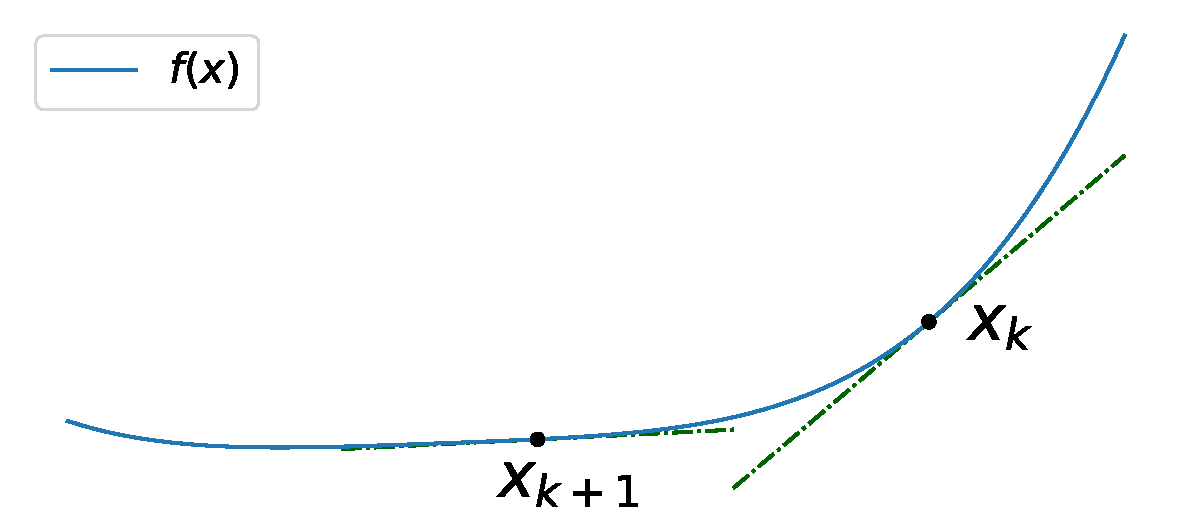
\includegraphics[width=\linewidth]{../imgs/modified_secant/trial_EXPLAIN.pdf}
        \subcaption{Available function and gradient data at $x_k$ and $x_{k+1}$.}
        \label{fig:msec_explain}
    \end{subfigure}%
    \hfill
    \begin{subfigure}[t]{0.33\textwidth}
        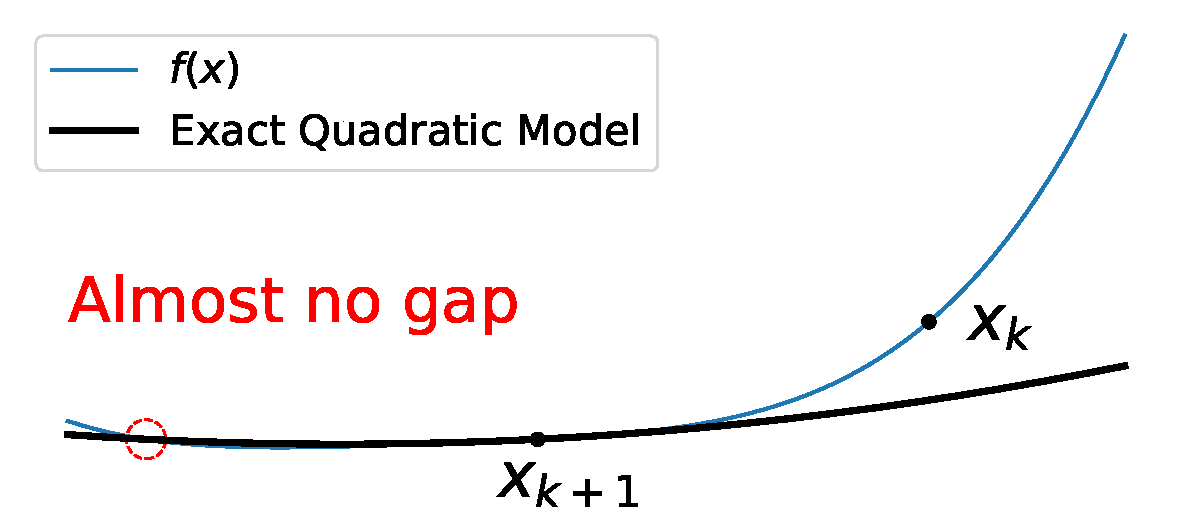
\includegraphics[width=\linewidth]{../imgs/modified_secant/trial_HESS.pdf}
        \subcaption{Ideal quadratic from the exact Hessian.}
        \label{fig:ideal_model}
    \end{subfigure}%
    \hfill
    \begin{subfigure}[t]{0.33\textwidth}
        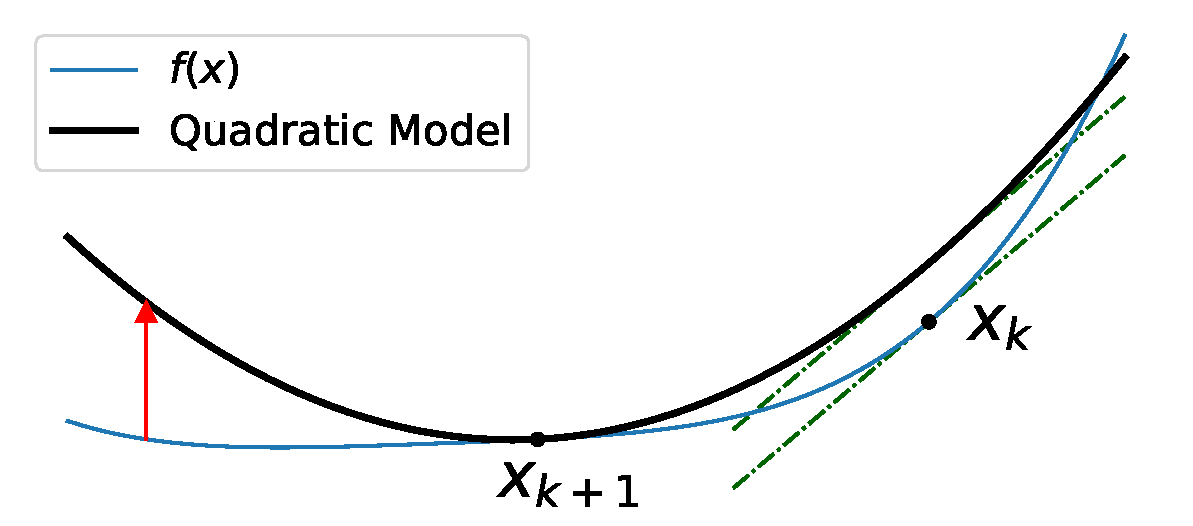
\includegraphics[width=\linewidth]{../imgs/modified_secant/trial_BFGS.pdf}
        \subcaption{Standard secant matches gradient but not $f(x_k)$.}
        \label{fig:standard_secant}
    \end{subfigure}
    \caption{
        \ifEn
            Motivation for modified secant equations. Combining function values with gradients (a) aims to approximate the ideal Newton model (b), while the standard secant update (c) omits $f(x_k)$ and can misestimate curvature.
        \else
            修正セカント方程式の動機。関数値と勾配を組み合わせることにより、理想的なニュートン法モデル (b) に近似することを目指しており、標準的なセカント更新 (c) は $f(x_k)$ を省略して曲率を誤推定する可能性があります。
        \fi
    }
    \label{fig:msec_overview}
\end{figure}

\ifEn
    We can overcome this limitation by utilizing the function values.
    The basic idea is illustrated in \cref{fig:cubic_interpolation}.
    Even when the gradients are the same at two points $x_k$ and $x_{k+1}$, natural interpolation of function values differs depending on the function values $f(x_k)$ and $f(x_{k+1})$.
    This observation motivates the modified secant condition, which incorporates function value information to improve Hessian approximation.
\else
    関数値を利用することでこの制限を克服できます。
    基本的な考え方は \cref{fig:cubic_interpolation} に示されています。
    2 点 $x_k$ と $x_{k+1}$ で勾配が同じであっても、関数値の自然な内挿は関数値 $f(x_k)$ と $f(x_{k+1})$ に応じて異なります。
    この観察は、関数値情報を取り込んでヘッセ行列の近似を改善する修正セカント条件の動機となります。
\fi

\begin{figure}[htbp]
    \centering
    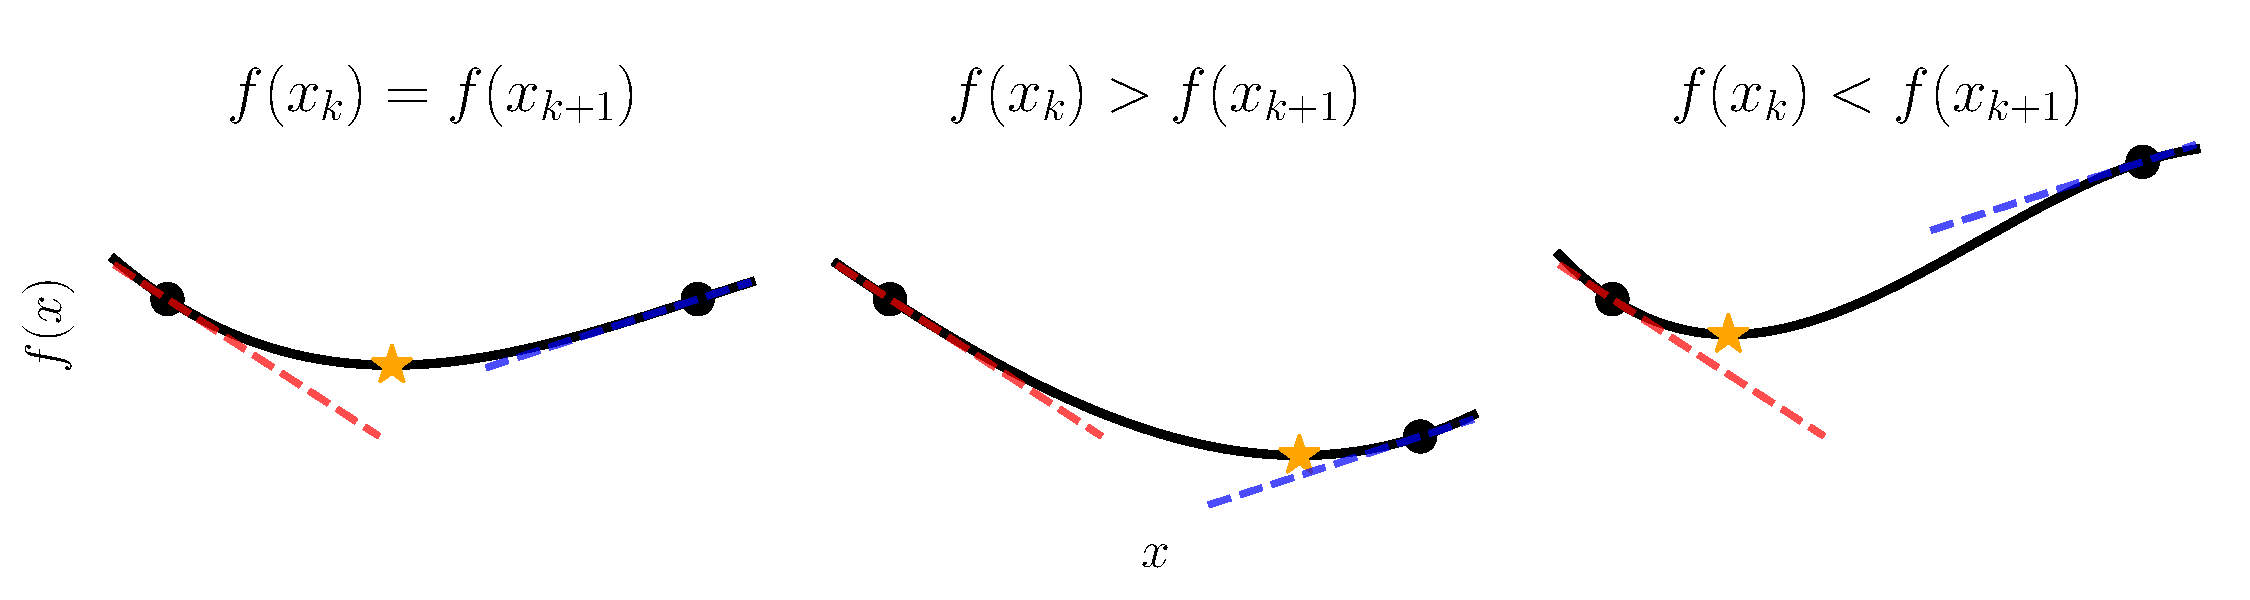
\includegraphics[width=\textwidth]{../imgs/modified_secant/cubic_interpolation.pdf}
    \caption{
        \ifEn
            Interpolation with identical gradients at $x_k$ and $x_{k+1}$ but different function values. This leads to distinct interpolants, highlighting the importance of incorporating function value information in Hessian approximation.
        \else
            $x_k$ と $x_{k+1}$ で同一の勾配を持つが異なる関数値による内挿。これは異なる内挿関数を生じさせ、ヘッセ行列の近似に関数値情報を組み込むことの重要性を強調しています。
        \fi
    }
    \label{fig:cubic_interpolation}
\end{figure}

\ifEn
    In the following, we present two well-known modified secant conditions.
\else
    以下では、2つの既知の修正セカント条件を提示します。
\fi

\ifEn
    \subsubsection{Function-Value-Based Modified Secant Condition}
\else
    \subsubsection{関数値ベースの修正セカント条件}
\fi
\label{subsubsec:yuan}

\ifEn
    The first modification incorporates the function value at the previous point into the quadratic model \citep{yuanModifiedBFGSAlgorithm1991,weiNewQuasiNewtonMethods2006, babaie-kafakiModifiedBFGSAlgorithm2011}.
    Let us consider an alternate model with a different approximate Hessian $B^{\mathrm{F}}_{k+1}$:
\else
    最初の修正は、前の点での関数値を二次モデルに組み込みます \citep{yuanModifiedBFGSAlgorithm1991,weiNewQuasiNewtonMethods2006, babaie-kafakiModifiedBFGSAlgorithm2011}。
    異なる近似ヘッセ行列 $B^{\mathrm{F}}_{k+1}$ を持つ別のモデルを考えましょう:
\fi
\begin{equation*}
    m_{k+1}^{\mathrm{F}}(x) = f(x_{k+1}) + \nabla f(x_{k+1})^\top (x - x_{k+1}) + \frac{1}{2} (x - x_{k+1})^\top B^{\mathrm{F}}_{k+1} (x - x_{k+1}).
\end{equation*}
\ifEn
    We require this model to satisfy
\else
    このモデルが以下を満たすことを要求します:
\fi
\begin{equation*}
    m^{\mathrm{F}}_{k+1}(x_k) = f(x_k),
\end{equation*}
\ifEn
    which enforces that the function value at the previous point is correctly modeled.
    This is the key idea behind function-value-based modified secant conditions.
\else
    これは前の点での関数値が正しくモデル化されることを保証します。
    これが関数値ベースの修正セカント条件の背後にある主要な考え方です。
\fi

\ifEn
    Let us derive the corresponding modified secant condition for $B^{\mathrm{F}}_{k+1}$.
    Substituting the definition of $m^{\mathrm{F}}_{k+1}$ and using $s_k = x_{k+1} - x_k$, the condition becomes
\else
    対応する修正セカント条件を $B^{\mathrm{F}}_{k+1}$ に対して導出しましょう。
    $m^{\mathrm{F}}_{k+1}$ の定義を代入し、$s_k = x_{k+1} - x_k$ を使用することで、条件は以下になります
\fi
\begin{align*}
    f(x_k) & = f(x_{k+1}) + \nabla f(x_{k+1})^\top (x_k - x_{k+1}) + \frac{1}{2} (x_k - x_{k+1})^\top B^{\mathrm{F}}_{k+1} (x_k - x_{k+1}) \\
           & = f(x_{k+1}) - \nabla f(x_{k+1})^\top s_k + \frac{1}{2} s_k^\top B^{\mathrm{F}}_{k+1} s_k.
\end{align*}
\ifEn
    Now, assume that the updated matrix has the form
\else
    次に、更新された行列が以下の形を持つと仮定します
\fi
\begin{equation*}
    B^{\mathrm{F}}_{k+1} s_k = y_k - \sigma^\mathrm{F}_k s_k,
\end{equation*}
\ifEn
    where $\sigma^\mathrm{F}_k \in \mathbb{R}$ is a scalar to be determined.
\else
    ここで、$\sigma^\mathrm{F}_k \in \mathbb{R}$ は決定する必要があるスカラーです。
\fi
Substituting this equation and using $s_k^\top B^{\mathrm{F}}_{k+1} s_k = s_k^\top y_k - \sigma^\mathrm{F}_k \lVert s_k \rVert^2$ gives
\begin{equation*}
    f(x_k) = f(x_{k+1}) - \nabla f(x_{k+1})^\top s_k + \frac{1}{2} s_k^\top y_k - \frac{\sigma^\mathrm{F}_k}{2} \lVert s_k \rVert^2.
\end{equation*}
\ifEn
    Solving for $\sigma^\mathrm{F}_k$ and using $y_k = \nabla f(x_{k+1}) - \nabla f(x_k)$, we obtain
\else
    $\sigma^\mathrm{F}_k$ について解き、$y_k = \nabla f(x_{k+1}) - \nabla f(x_k)$ を使用することで、以下を得ます
\fi
\begin{align*}
    \sigma^\mathrm{F}_k & = \frac{2(f(x_{k+1}) - f(x_k)) - (2\nabla f(x_{k+1}) - y_k)^\top s_k}{\lVert s_k \rVert^2}           \\
                        & = \frac{2(f(x_{k+1}) - f(x_k)) - (\nabla f(x_{k+1}) + \nabla f(x_k))^\top s_k}{\lVert s_k \rVert^2}.
\end{align*}
\ifEn
    Therefore, the modified secant condition becomes
\else
    したがって、修正セカント条件は以下になります
\fi
\begin{equation*}
    B^{\mathrm{F}}_{k+1} s_k = y_k + \frac{2(f(x_k) - f(x_{k+1})) + (\nabla f(x_{k+1}) + \nabla f(x_k))^\top s_k}{\lVert s_k \rVert^2} s_k.
\end{equation*}
\ifEn
    To preserve the possibility of maintaining positive definiteness under a BFGS-type update when $s_k^\top y_k > 0$, we can modify the formula by taking the maximum with zero in the numerator.
\else
    $s_k^\top y_k > 0$ の場合に BFGS 型更新の下で正定性を保つ可能性を保存するために、分子でゼロとの最大値を取ることでこの公式を修正できます。
\fi
\begin{equation*}
    B^{\mathrm{F}'}_{k+1} s_k = y_k + \frac{\max(0, 2(f(x_k) - f(x_{k+1})) + (\nabla f(x_{k+1}) + \nabla f(x_k))^\top s_k)}{\lVert s_k \rVert^2} s_k.
\end{equation*}

\ifEn
    This is the function-value-based modified secant condition.
    Unlike the standard secant condition, this formulation ensures that the quadratic model matches not only the function value at the previous point but also the gradients at both points.
    Refer to \cref{fig:yuan_msec} for an illustration.
\else
    これが関数値ベースの修正セカント条件です。
    標準的なセカント条件とは異なり、この定式化は二次モデルが前の点での関数値だけでなく、両方の点での勾配と一致することを保証します。
    説明については \cref{fig:yuan_msec} を参照してください。
\fi

\begin{figure}[t]
    \centering
    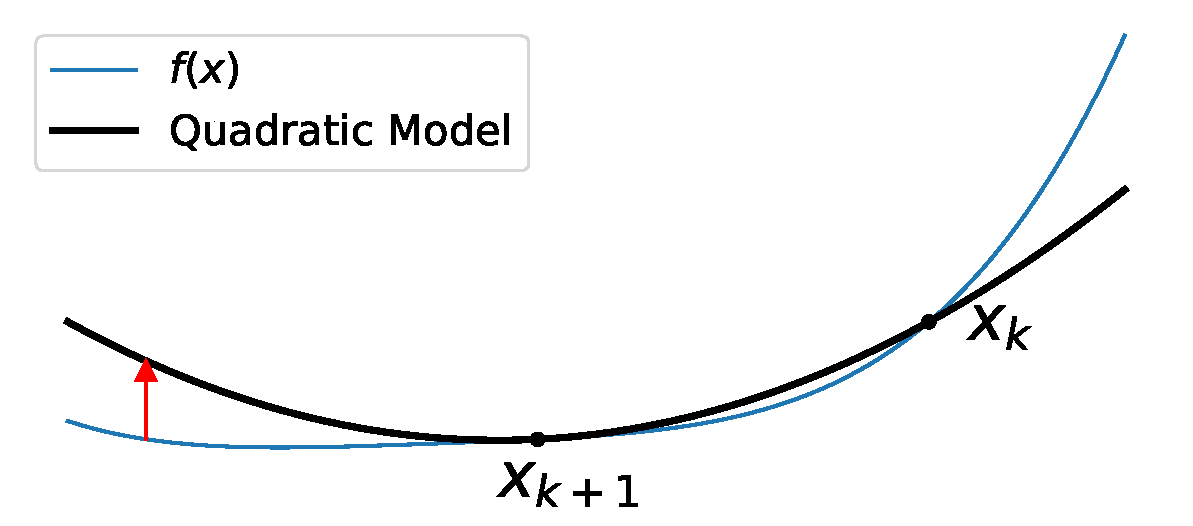
\includegraphics[width=0.7\textwidth]{../imgs/modified_secant/trial_2.pdf}
    \caption{
        \ifEn
            Function-value-based modified secant equation. The modified secant equation $B^\mathrm{F}_k s_k = y_k + \sigma^\mathrm{F}_k s_k$ constructs a quadratic model that satisfies the function value condition $m^{\mathrm{F}}_k(x_{k-1}) = f(x_{k-1})$ at the previous point. This differs from the standard secant equation, which only matches gradients but not function values.
        \else
            関数値ベースの修正セカント方程式。修正セカント方程式 $B^\mathrm{F}_k s_k = y_k + \sigma^\mathrm{F}_k s_k$ は、前の点での関数値条件 $m^{\mathrm{F}}_k(x_{k-1}) = f(x_{k-1})$ を満たす二次モデルを構築します。これは勾配のみを照合し、関数値を照合しない標準的なセカント方程式とは異なります。
        \fi
    }
    \label{fig:yuan_msec}
\end{figure}

\ifEn
    \subsubsection{Cubic-Augmented Modified Secant Condition}
\else
    \subsubsection{3次項付き修正セカント条件}
\fi
\label{subsubsec:zhang}

\ifEn
    The second modification introduces a cubic term to the model, allowing simultaneous satisfaction of both function value and gradient matching at the previous point \citep{zhangNewQuasiNewtonEquation1999, zhangPropertiesNumericalPerformance2001,yabeLocalSuperlinearConvergence2007}.
\else
    2 番目の修正はモデルに 3 次項を導入し、前の点での関数値と勾配の両方の一致を同時に満たすことを可能にします \citep{zhangNewQuasiNewtonEquation1999, zhangPropertiesNumericalPerformance2001,yabeLocalSuperlinearConvergence2007}。
\fi
\ifEn
    Let $T_{k+1} \in \mathbb{R}^{n \times n \times n}$ be the third-order derivative tensor of $f$ at $x_{k+1}$ such that
\else
    $T_{k+1} \in \mathbb{R}^{n \times n \times n}$ を $x_{k+1}$ での $f$ の3階微分テンソルとし、以下を満たすものとします
\fi
\begin{equation*}
    s_k^\top (T_{k+1} s_k) s_k = \sum_{i,j,l=1}^n \partial_{x_i x_j x_l} f(x_{k+1}) s_k^{(i)} s_k^{(j)} s_k^{(l)},
\end{equation*}
\ifEn
    where $\partial_{x_i x_j x_l} f$ denotes the third derivative of $f$ with respect to $x_i$, $x_j$, and $x_l$, and $s_k^{(i)}$ is the $i$-th component of the vector $s_k$.
    We introduced this tensor solely for analysis purposes, and it will be eliminated from the final formula.
\else
    ここで、$\partial_{x_i x_j x_l} f$ は $f$ の $x_i$、$x_j$、および $x_l$ に対する3階微分を表し、$s_k^{(i)}$ はベクトル $s_k$ の第 $i$ 成分です。
    このテンソルは分析目的でのみ導入され、最終公式から除去されます。
\fi

\ifEn
    By incorporating this tensor term, we can define the following cubic-augmented model:
\else
    このテンソル項を組み込むことにより、以下の3次拡張モデルを定義できます:
\fi
\begin{align*}
    m^\mathrm{C}_{k+1}(x) ={} & f(x_{k+1}) + \nabla f(x_{k+1})^\top (x - x_{k+1}) + \frac{1}{2} (x - x_{k+1})^\top B_{k+1}^{\mathrm{C}} (x - x_{k+1}) \\
                              & + \frac{1}{6}(x - x_{k+1})^\top (T_{k+1} (x - x_{k+1})) (x - x_{k+1}).
\end{align*}
\ifEn
    With this model, we can enforce both function value and gradient matching at the previous point $x_k$.
    Specifically, we require
\else
    このモデルを使用して、前の点 $x_k$ での関数値と勾配の両方の一致を強制できます。
    具体的には、以下を要求します:
\fi
\begin{equation*}
    \begin{dcases}
        m^\mathrm{C}_{k+1}(x_k) = f(x_k) \\
        \nabla m^\mathrm{C}_{k+1}(x_k) = \nabla f(x_k)
    \end{dcases}
\end{equation*}
\ifEn
    By substituting the definition of $m^\mathrm{C}_{k+1}$ and using $s_k = x_{k+1} - x_k$, we can rewrite these conditions as
\else
    $m^\mathrm{C}_{k+1}$ の定義を代入し、$s_k = x_{k+1} - x_k$ を使用することで、これらの条件を以下のように書き直せます
\fi
\begin{align*}
    f(x_k)        & = f(x_{k+1}) - s_k^\top \nabla f(x_{k+1}) + \frac{1}{2} s_k^\top B^\mathrm{C}_{k+1} s_k - \frac{1}{6} s_k^\top (T_{k+1} s_k) s_k, \\
    \nabla f(x_k) & = \nabla f(x_{k+1}) - B^\mathrm{C}_{k+1} s_k + \frac{1}{2} (T_{k+1} s_k) s_k.
\end{align*}
\ifEn
    Rearranging and multiplying both sides by $3$ for the first equation, and taking the inner product with $s_k$ for the second equation, we have
\else
    第1の方程式の両辺に3を乗じて整理し、第2の方程式については $s_k$ との内積をとることで、以下が得られます
\fi
\begin{align*}
    3(f(x_k) - f(x_{k+1})) +3 s_k^\top \nabla f(x_{k+1}) & = \frac{3}{2} s_k^\top B^{\mathrm{C}}_{k+1} s_k - \frac{1}{2} s_k^\top (T_{k+1} s_k) s_k, \\
    -s_k^\top y_k                                        & = -s_k^\top B^{\mathrm{C}}_{k+1} s_k + \frac{1}{2} s_k^\top (T_{k+1} s_k) s_k.
\end{align*}
\ifEn
    By summing up and using $y_k = \nabla f(x_{k+1}) - \nabla f(x_k)$, we eliminate the tensor term and obtain the scalar identity
\else
    合計し、$y_k = \nabla f(x_{k+1}) - \nabla f(x_k)$ を使用することで、テンソル項を除去し、以下のスカラー恒等式を得ます
\fi
\begin{equation*}
    3(f(x_k) - f(x_{k+1}))
    + \frac{3}{2} s_k^\top (\nabla f(x_{k+1}) + \nabla f(x_k)) + \frac{1}{2} s_k^\top y_k
    = \frac{1}{2} s_k^\top B^{\mathrm{C}}_{k+1} s_k.
\end{equation*}
\ifEn
    Assume again that $B^{\mathrm{C}}_{k+1} s_k$ is a linear combination of $y_k$ and $s_k$, i.e., $B^{\mathrm{C}}_{k+1} s_k = y_k + \sigma^\mathrm{C}_k s_k$ for some scalar $\sigma^\mathrm{C}_k$.
    Then, the previous equation yields
\else
    $B^{\mathrm{C}}_{k+1} s_k$ が $y_k$ と $s_k$ の線形結合であると仮定します。つまり、スカラー $\sigma^\mathrm{C}_k$ に対して $B^{\mathrm{C}}_{k+1} s_k = y_k + \sigma^\mathrm{C}_k s_k$ です。
    そうすると、前の方程式は以下を与えます
\fi
\begin{equation*}
    \sigma^\mathrm{C}_k = \frac{6(f(x_k) - f(x_{k+1})) + 3 s_k^\top (\nabla f(x_k) + \nabla f(x_{k+1}))}{\lVert s_k \rVert^2}.
\end{equation*}
\ifEn
    Thus, the modified secant condition becomes
\else
    したがって、修正セカント条件は以下になります
\fi
\begin{equation*}
    B^{\mathrm{C}}_{k+1} s_k = y_k + \frac{6(f(x_k) - f(x_{k+1})) + 3 s_k^\top (\nabla f(x_k) + \nabla f(x_{k+1}))}{\lVert s_k \rVert^2} s_k.
\end{equation*}

\ifEn
    This is a cubic-augmented modified secant condition. Unlike the function-value-based quadratic modification, this formulation allows simultaneous satisfaction of both the function value and gradient conditions at the previous point through the introduction of the tensor term.
    Refer to \cref{fig:zhang_models} for an illustration.
\else
    これが3次拡張修正セカント条件です。関数値ベースの二次修正とは異なり、この定式化はテンソル項の導入を通じて前の点での関数値条件と勾配条件の両方を同時に満たすことを可能にします。
    説明については \cref{fig:zhang_models} を参照してください。
\fi

\begin{figure}[t]
    \centering
    \begin{subfigure}[t]{0.49\textwidth}
        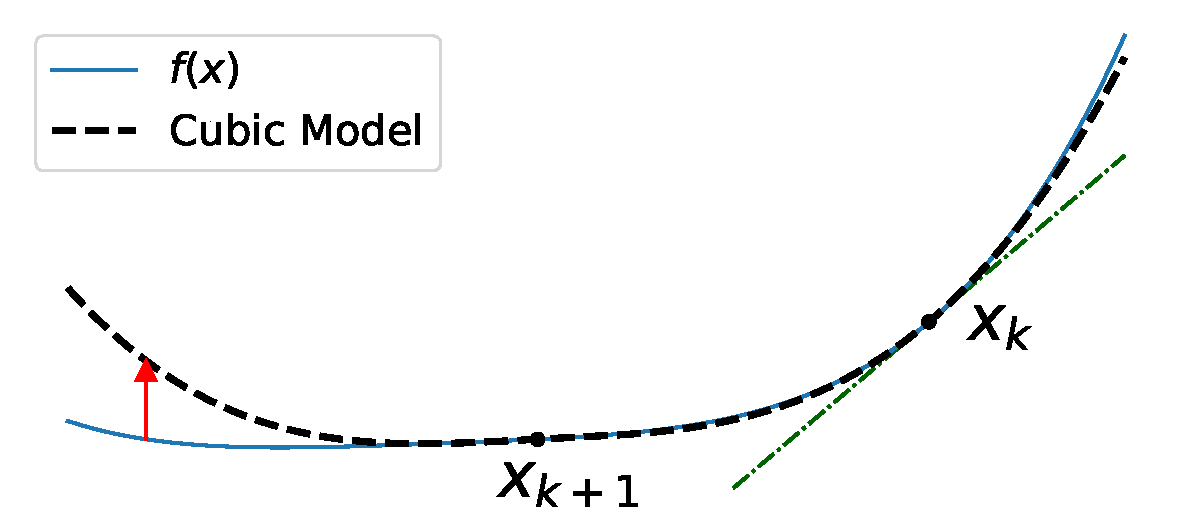
\includegraphics[width=\linewidth]{../imgs/modified_secant/trial_1_cubic.pdf}
        \subcaption{Cubic-augmented modified secant.}
        \label{fig:zhang_cubic}
    \end{subfigure}%
    \hfill
    \begin{subfigure}[t]{0.49\textwidth}
        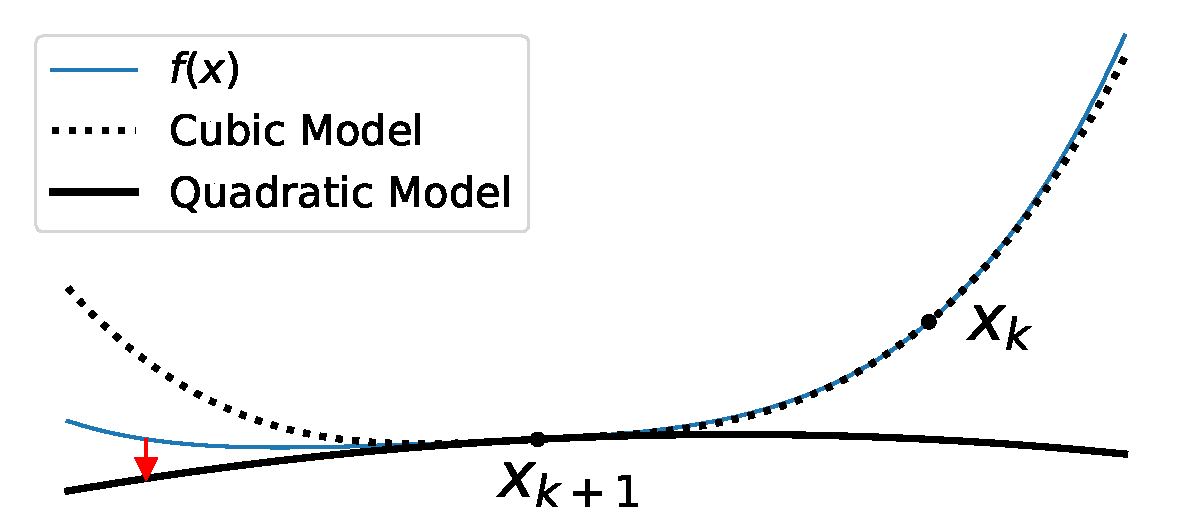
\includegraphics[width=\linewidth]{../imgs/modified_secant/trial_1_quadratic.pdf}
        \subcaption{Quadratic expansion of the cubic-augmented model.}
        \label{fig:zhang_quadratic}
    \end{subfigure}
    \caption{
        \ifEn
            Cubic-augmented modified secant equation. In \cref{fig:zhang_cubic}, by incorporating a cubic term $\eta \lVert x - x_k \rVert^3$ in the model, the modified secant equation $B^\mathrm{C}_k s_k = y_k + \sigma^\mathrm{C}_k s_k$ enables simultaneous satisfaction of both conditions at the previous point. In \cref{fig:zhang_quadratic}, while the cubic model satisfies both function value and gradient conditions, its underlying quadratic component may be indefinite or negative definite.
        \else
            3次拡張修正セカント方程式。\cref{fig:zhang_cubic} では、3次項 $\eta \lVert x - x_k \rVert^3$ をモデルに組み込むことにより、修正セカント方程式 $B^\mathrm{C}_k s_k = y_k + \sigma^\mathrm{C}_k s_k$ は前の点での両方の条件を同時に満たすことを可能にします。\cref{fig:zhang_quadratic} では、3次モデルは関数値と勾配の条件の両方を満たしていますが、その基礎となる二次成分は不定値または負定値である可能性があります。
        \fi
    }
    \label{fig:zhang_models}
\end{figure}

\ifEn
    \subsection{Other Curvature Storage Methods}
\else
    \subsection{その他の曲率保存方法}
\fi

\ifEn
    For storing the curvature information, there are several topics.
    Agg-BFGS \citep{berahasLimitedmemoryBFGSDisplacement2022} is an alternative approach to managing curvature information by aggregating data rather than discarding the oldest information and adding the newest.
\else
    曲率情報を保存するために、いくつかのトピックがあります。
    Agg-BFGS \citep{berahasLimitedmemoryBFGSDisplacement2022} は、最も古い情報を破棄して最新のものを追加するのではなく、データを集約することにより曲率情報を管理する別のアプローチです。
\fi
\ifEn
    Multi-Secant \citep{leeAdvancingMultiSecantQuasiNewton2025} extends the secant condition framework by maintaining multiple pairs of step and gradient difference vectors. In the standard formulation, we define
\else
    Multi-Secant \citep{leeAdvancingMultiSecantQuasiNewton2025} は、複数のステップと勾配差ベクトルのペアを維持することにより、セカント条件フレームワークを拡張します。標準的な定式化では、以下を定義します
\fi
\begin{equation*}
    s_i = x_{i+1} - x_i, \quad y_i = \nabla f(x_{i+1}) - \nabla f(x_i). \quad (i = k-m, \ldots, k)
\end{equation*}
\ifEn
    An alternative anchored formulation centers all vectors at the most recent iterate:
\else
    別の固定点型定式化は、すべてのベクトルを最新の反復で中心化します:
\fi
\begin{equation*}
    s_i = x_{k+1} - x_i, \quad y_i = \nabla f(x_{k+1}) - \nabla f(x_i). \quad (i = k-m, \ldots, k)
\end{equation*}
\ifEn
    This anchored approach provides a different perspective on utilizing historical information for improved Hessian approximation.
\else
    この固定点型アプローチは、改善されたヘッセ行列の近似のための履歴情報の利用に関する異なる観点を提供します。
\fi

\ifSubfilesClassLoaded{
    \bibliographystyle{plainnat}
    \bibliography{../L-BFGS.bib}
}{}

\end{document}
